% =============================================================================
%  NGEN-AI 2026 - Paper 15, Session 7
%  Robust Function Calling for LLM Agents Under Interface Drift
%  Build: latexmk -pdf -outdir=tmp presentation.tex   (pdflatex)
% =============================================================================
\documentclass[aspectratio=169,11pt]{beamer}

\usepackage[T1]{fontenc}
\usepackage[utf8]{inputenc}
\usepackage[sfdefault,semibold]{inter}
\usepackage{plex-mono}
\usepackage{microtype}
\usepackage[document]{ragged2e}
\usepackage{booktabs}
\usepackage{array}
\usepackage{xspace}
\usepackage{tikz}
\usetikzlibrary{arrows.meta,calc,positioning,shapes.geometric}
\usepackage{hyperref}

% Slides read better unhyphenated.
\hyphenpenalty=10000
\exhyphenpenalty=10000
\tolerance=3000

\newcommand{\method}{SchemaShield-Lite\xspace}

% ---------------------------------------------------------------- design tokens
\definecolor{Canvas}{HTML}{FCFCFA}
\definecolor{Ink}{HTML}{16191F}
\definecolor{Body}{HTML}{3A414D}
\definecolor{Mute}{HTML}{7B8492}
\definecolor{Line}{HTML}{E3E4E0}
\definecolor{Accent}{HTML}{0E6E7D}
\definecolor{AccentIn}{HTML}{DCEBED}
\definecolor{Warm}{HTML}{BF553B}
\definecolor{WarmIn}{HTML}{F7E6E0}
\definecolor{Slate}{HTML}{AAB1BC}
\definecolor{Dark}{HTML}{14171D}
\definecolor{DarkMute}{HTML}{8D96A4}

\setbeamercolor{background canvas}{bg=Canvas}
\setbeamercolor{normal text}{fg=Body}
\setbeamercolor{frametitle}{fg=Ink}
\setbeamercolor{structure}{fg=Accent}
\setbeamerfont{normal text}{size=\fontsize{12}{15.5}}
\setbeamersize{text margin left=1.1cm,text margin right=1.1cm}

\setbeamertemplate{navigation symbols}{}
\setbeamertemplate{itemize item}{\color{Accent}\raise0.22ex\hbox{\rule{0.5ex}{0.5ex}}}
\setbeamertemplate{itemize subitem}{\color{Mute}\raise0.22ex\hbox{\rule{0.4ex}{0.4ex}}}

% Frame title: short accent tick above the title, no rule below.
\setbeamerfont{frametitle}{series=\bfseries,size=\fontsize{17}{20}}
\setbeamertemplate{frametitle}{%
  \vspace{0.22cm}%
  {\color{Accent}\rule{0.55cm}{2pt}}\par%
  \vspace{0.10cm}%
  \insertframetitle\par%
}

\setbeamerfont{footline}{size=\fontsize{6.8}{8}}
\setbeamertemplate{footline}{%
  \leavevmode%
  \hbox{%
    \begin{beamercolorbox}[wd=.80\paperwidth,ht=0.30cm,dp=0.18cm,leftskip=1.1cm]{footline}%
      \color{Mute}NGEN-AI 2026\, \textperiodcentered\, Session 7\, \textperiodcentered\, Paper 15
    \end{beamercolorbox}%
    \begin{beamercolorbox}[wd=.20\paperwidth,ht=0.30cm,dp=0.18cm,rightskip=1.1cm plus1fil]{footline}%
      \color{Mute}\hfill\insertframenumber
    \end{beamercolorbox}%
  }%
}

% ---------------------------------------------------------------------- helpers
\newcommand{\eyebrow}[1]{%
  {\color{Mute}\fontsize{8}{10}\selectfont\bfseries\textls[100]{\MakeUppercase{#1}}}\par}
\newcommand{\eyebrowon}[2]{%
  {\color{#1}\fontsize{8}{10}\selectfont\bfseries\textls[100]{\MakeUppercase{#2}}}\par}

% Headline statistic with caption underneath.
\newcommand{\stat}[2]{%
  {\color{Accent}\fontsize{24}{27}\selectfont\bfseries #1}\par
  \vspace{0.05cm}{\color{Mute}\fontsize{9}{11.5}\selectfont #2}\par}

% Thin divider rule.
\newcommand{\hairline}{{\color{Line}\rule{\textwidth}{0.6pt}}\par}

% Full-bleed dark background for statement frames.
\newcommand{\darkbleed}{%
  \begin{tikzpicture}[remember picture,overlay]
    \fill[Dark] (current page.north west) rectangle (current page.south east);
  \end{tikzpicture}}

% One row of a horizontal bar chart. \barfont sets the label size per slide.
%   #1 y  #2 category label  #3 value label  #4 bar length (cm)  #5 bar colour
\newcommand{\barfont}{\fontsize{9.5}{12}\selectfont}
\newcommand{\barrow}[5]{%
  \node[anchor=east,text=Body,font=\barfont] at (-0.15,#1) {#2};
  \fill[#5] (0,{#1-0.145}) rectangle ({#4},{#1+0.145});
  \node[anchor=west,text=Ink,font=\bfseries\barfont] at ({#4+0.14},#1) {#3};}
\newcommand{\barrowhi}[5]{%
  \node[anchor=east,text=Ink,font=\bfseries\barfont] at (-0.15,#1) {#2};
  \fill[#5] (0,{#1-0.145}) rectangle ({#4},{#1+0.145});
  \node[anchor=west,text=Ink,font=\bfseries\barfont] at ({#4+0.14},#1) {#3};}

% Monospace code.
\newcommand{\code}[1]{{\ttfamily\fontsize{8.4}{11.4}\selectfont #1}}

\begin{document}

% == 1 == Title ================================================================
\begin{frame}[plain]
  \darkbleed
  \begin{tikzpicture}[remember picture,overlay]
    \fill[Accent] ([xshift=1.1cm,yshift=-1.30cm]current page.north west)
      rectangle ([xshift=1.66cm,yshift=-1.37cm]current page.north west);
    \fill[Accent] ([xshift=0cm,yshift=0.55cm]current page.south east)
      rectangle ([xshift=-2.4cm,yshift=0.49cm]current page.south east);
  \end{tikzpicture}

  \vspace{0.22cm}
  \eyebrowon{DarkMute}{NGEN-AI 2026 \ \textperiodcentered\ \ Session 7 \ \textperiodcentered\ \ Paper 15}

  \vspace{0.86cm}
  {\color{Canvas}\fontsize{25}{29}\selectfont\bfseries
    Robust Function Calling\\[0.04cm]
    for LLM Agents\\[0.04cm]
    Under Interface Drift\par}

  \vspace{0.40cm}
  {\color{DarkMute}\fontsize{12}{15.5}\selectfont
    Training-free validation and one-shot repair\\for tool interfaces that change after deployment\par}

  \vfill
  {\color{Canvas}\fontsize{10.5}{13}\selectfont\bfseries
    Aniruddha Chattopadhyay \quad Kanishka Halder \quad Partha Sarathi Roy\par}
  \vspace{0.10cm}
  {\color{DarkMute}\fontsize{9}{11}\selectfont Independent Researchers, Bangalore, India\par}
  \vspace{0.52cm}

  \note{%
    0:00-0:40. Open with the deployment problem: tool semantics can stay fixed while the textual interface changes underneath an agent. Ask whether a small runtime layer can recover reliability without retraining.\\
    [Sources] Paper 15 title block; NGEN-AI 2026 program page.
  }
\end{frame}

% == 2 == What interface drift is ==============================================
\begin{frame}{Tool semantics stay fixed. Interfaces move.}
  \vspace{0.26cm}
  \begin{columns}[T,onlytextwidth]
    \begin{column}{0.35\textwidth}
      \eyebrow{Stable intent}
      \vspace{0.22cm}
      {\color{Ink}\fontsize{16}{19.5}\selectfont\bfseries Find the same\\customer orders\par}
      \vspace{0.28cm}
      {\fontsize{10.5}{14}\selectfont
        The API behaves exactly as before. The agent still needs the same tool and the same information.\par}
    \end{column}

    \begin{column}{0.59\textwidth}
      \eyebrow{What moved}
      \vspace{0.10cm}
      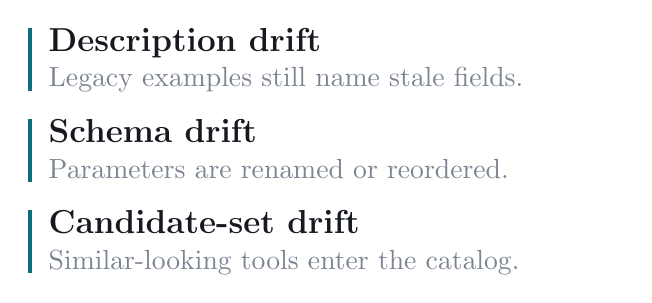
\begin{tikzpicture}[x=1cm,y=1cm]
        \foreach \yy/\ttl/\sub in {%
          3.44/{Description drift}/{Legacy examples still name stale fields.},
          2.28/{Schema drift}/{Parameters are renamed or reordered.},
          1.12/{Candidate-set drift}/{Similar-looking tools enter the catalog.}}{%
          \fill[Accent] (0,{\yy-0.80}) rectangle (0.05,{\yy});
          \node[anchor=north west,text width=7.3cm,inner sep=0] at (0.26,\yy) {%
            {\color{Ink}\fontsize{12.5}{15}\selectfont\bfseries \ttl}\par
            \vspace{0.03cm}{\color{Mute}\fontsize{10}{12.5}\selectfont \sub}};}
      \end{tikzpicture}
    \end{column}
  \end{columns}

  \vspace{0.16cm}
  \hairline
  \vspace{0.12cm}
  {\fontsize{10.5}{13.5}\selectfont
    Every edit is \textbf{semantics-preserving}. Nothing the tool does changed --- only the contract the model reads.\par}

  \note{%
    0:40-1:55. Define interface drift as benign, semantics-preserving change to descriptions, schemas, or the visible candidate set. Stress that this is a post-deployment contract problem, not a change in what the tool does, and not a tool outage.\\
    [Sources] Paper 15, Sections 1 and 3.
  }
\end{frame}

% == 3 == Concrete example =====================================================
\begin{frame}{What that actually breaks}
  \vspace{0.02cm}
  \eyebrow{Illustrative example}
  \vspace{0.06cm}

  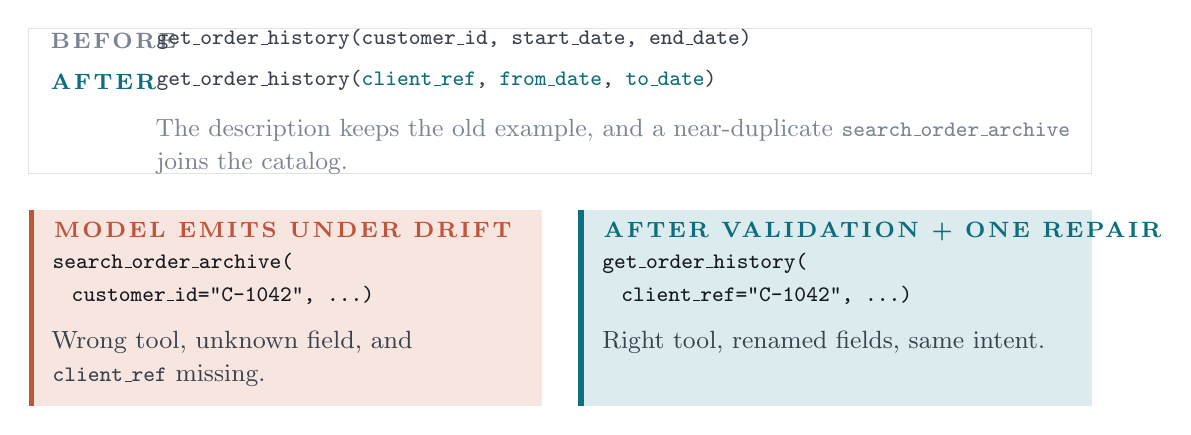
\begin{tikzpicture}[x=1cm,y=1cm]
    % ---- the interface, before and after -------------------------------------
    \fill[white] (0,3.16) rectangle (13.5,5.00);
    \draw[Line,line width=0.6pt] (0,3.16) rectangle (13.5,5.00);

    \node[anchor=west,inner sep=0] at (0.26,4.84)
      {{\color{Mute}\fontsize{8}{10}\selectfont\bfseries\textls[100]{BEFORE}}};
    \node[anchor=west,inner sep=0] at (1.62,4.86)
      {\code{\color{Body}get\_order\_history(customer\_id, start\_date, end\_date)}};

    \node[anchor=west,inner sep=0] at (0.26,4.32)
      {{\color{Accent}\fontsize{8}{10}\selectfont\bfseries\textls[100]{AFTER}}};
    \node[anchor=west,inner sep=0] at (1.62,4.34)
      {\code{\color{Body}get\_order\_history({\color{Accent}\bfseries client\_ref}, {\color{Accent}\bfseries from\_date}, {\color{Accent}\bfseries to\_date})}};

    \node[anchor=north west,inner sep=0,text width=11.6cm] at (1.62,3.86)
      {{\color{Mute}\fontsize{9}{11.5}\selectfont
        The description keeps the old example, and a near-duplicate \code{search\_order\_archive} joins the catalog.}};

    % ---- what the model emits ------------------------------------------------
    \fill[WarmIn] (0,0.20) rectangle (6.52,2.70);
    \fill[Warm]   (0,0.20) rectangle (0.07,2.70);
    \node[anchor=north west,inner sep=0] at (0.30,2.54)
      {{\color{Warm}\fontsize{8}{10}\selectfont\bfseries\textls[100]{MODEL EMITS UNDER DRIFT}}};
    \node[anchor=north west,inner sep=0,text width=5.9cm,align=left] at (0.30,2.16)
      {\code{\color{Ink}search\_order\_archive(\\\hspace*{2ex}customer\_id="C-1042", ...)}};
    \node[anchor=north west,inner sep=0,text width=5.9cm] at (0.30,1.16)
      {{\color{Body}\fontsize{9}{12}\selectfont
        Wrong tool, unknown field, and \code{client\_ref} missing.}};

    % ---- what repair emits ---------------------------------------------------
    \fill[AccentIn] (6.98,0.20) rectangle (13.5,2.70);
    \fill[Accent]   (6.98,0.20) rectangle (7.05,2.70);
    \node[anchor=north west,inner sep=0] at (7.28,2.54)
      {{\color{Accent}\fontsize{8}{10}\selectfont\bfseries\textls[100]{AFTER VALIDATION + ONE REPAIR}}};
    \node[anchor=north west,inner sep=0,text width=5.9cm,align=left] at (7.28,2.16)
      {\code{\color{Ink}get\_order\_history(\\\hspace*{2ex}client\_ref="C-1042", ...)}};
    \node[anchor=north west,inner sep=0,text width=5.9cm] at (7.28,1.16)
      {{\color{Body}\fontsize{9}{12}\selectfont
        Right tool, renamed fields, same intent.}};
  \end{tikzpicture}

  \note{%
    1:55-3:20. Make the failure concrete. The rename is semantics-preserving, but the stale description example and the near-duplicate tool push the model to the wrong call. Say clearly that this example is illustrative, built to show the mechanism, not a verbatim benchmark trace.\\
    [Sources] Paper 15, Section 3 drift operators; Section 6.6 residual mismatch types.
  }
\end{frame}

% == 4 == How we measure ========================================================
\begin{frame}{How we measure it}
  \vspace{0.16cm}
  \begin{columns}[T,onlytextwidth]
    \begin{column}{0.44\textwidth}
      \eyebrow{Three stages per example}
      \vspace{0.12cm}
      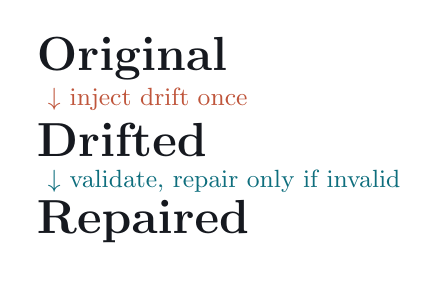
\begin{tikzpicture}[x=1cm,y=1cm]
        \node[anchor=west,text=Ink,font=\bfseries\fontsize{16}{19}\selectfont] at (0,2.94) {Original};
        \node[anchor=west,text=Warm,font=\fontsize{9.5}{12}\selectfont]        at (0.14,2.42)
          {$\downarrow$\hspace{0.35em}inject drift once};
        \node[anchor=west,text=Ink,font=\bfseries\fontsize{16}{19}\selectfont] at (0,1.90) {Drifted};
        \node[anchor=west,text=Accent,font=\fontsize{9.5}{12}\selectfont]      at (0.14,1.38)
          {$\downarrow$\hspace{0.35em}validate, repair only if invalid};
        \node[anchor=west,text=Ink,font=\bfseries\fontsize{16}{19}\selectfont] at (0,0.86) {Repaired};
      \end{tikzpicture}
      \vspace{0.06cm}
      {\fontsize{10}{13}\selectfont
        Scoring all three separates what drift \emph{breaks} from what repair \emph{recovers}.\par}
    \end{column}

    \begin{column}{0.50\textwidth}
      \eyebrow{The primary protocol is non-oracle}
      \vspace{0.24cm}
      {\fontsize{10}{13}\selectfont
      \begin{itemize}\setlength\itemsep{0.17cm}
        \item Sees the user context and the model's own output
        \item Sees only the tools visible at runtime
        \item \textbf{Never} sees the benchmark's gold tool
        \item No training, no persistent prompt update
      \end{itemize}}
      \vspace{0.20cm}
      {\color{Mute}\fontsize{9.5}{12}\selectfont
        Oracle-constrained runs appear later as upper bounds only.\par}
    \end{column}
  \end{columns}

  \note{%
    3:20-4:30. Clarify the non-oracle constraint: a deployed system does not know which tool the benchmark expects. It sees the live catalog, the generated call, and validation errors. Oracle runs are mechanism diagnostics, not deployment evidence.\\
    [Sources] Paper 15, Sections 3 and 5.4.
  }
\end{frame}

% == 5 == The method ============================================================
\begin{frame}{\method: validate, then repair once}
  \vspace{0.26cm}
  \centering
  \resizebox{\textwidth}{!}{%
  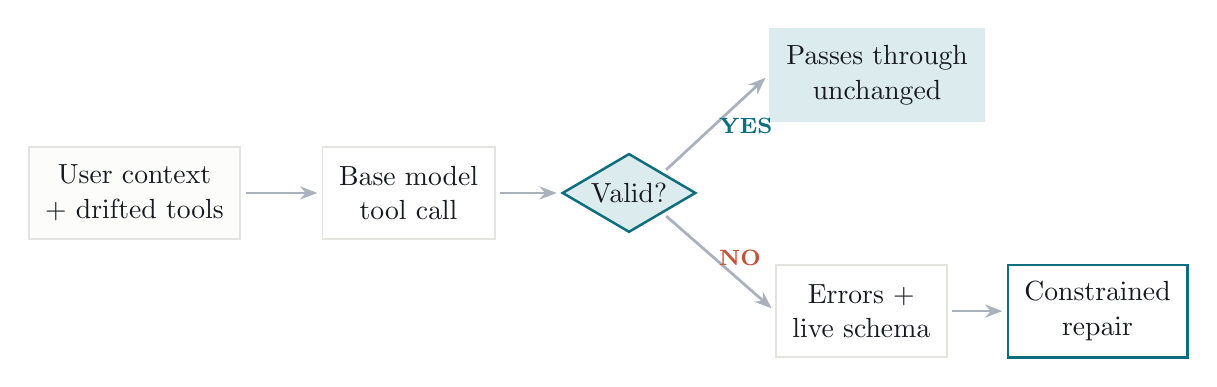
\begin{tikzpicture}[x=1cm,y=1cm,
      every node/.style={font=\fontsize{10}{12.5}\selectfont,text=Ink},
      box/.style={draw=Line,line width=0.7pt,fill=white,minimum height=1.16cm,
                  align=center,inner sep=6pt},
      flow/.style={-{Stealth[length=2.2mm]},line width=1.0pt,draw=Slate,
                   shorten >=1.5pt,shorten <=1.5pt}]
    \node[box,fill=Canvas]                  (ctx)  at (1.62,2.55) {User context\\+ drifted tools};
    \node[box]                              (base) at (5.10,2.55) {Base model\\tool call};
    \node[diamond,aspect=2.1,draw=Accent,line width=0.9pt,fill=AccentIn,
          minimum height=1.0cm,align=center,inner sep=1pt] (chk) at (7.90,2.55) {Valid?};
    \node[box,fill=AccentIn,draw=AccentIn]  (pass) at (11.05,4.05) {Passes through\\unchanged};
    \node[box]                              (err)  at (10.85,1.05) {Errors +\\live schema};
    \node[box,draw=Accent,line width=0.9pt] (rep)  at (13.85,1.05) {Constrained\\repair};

    \draw[flow] (ctx.east)  -- (base.west);
    \draw[flow] (base.east) -- (chk.west);
    \draw[flow] (chk.north east) -- (pass.west);
    \draw[flow] (chk.south east) -- (err.west);
    \draw[flow] (err.east)  -- (rep.west);

    \node[anchor=south west,text=Accent,font=\bfseries\fontsize{8.5}{10}\selectfont] at (8.92,3.18) {YES};
    \node[anchor=north west,text=Warm,font=\bfseries\fontsize{8.5}{10}\selectfont]   at (8.92,1.94) {NO};
  \end{tikzpicture}}

  \vspace{0.34cm}
  \begin{columns}[T,onlytextwidth]
    \begin{column}{0.485\textwidth}
      \hairline\vspace{0.10cm}
      {\fontsize{9.5}{12.5}\selectfont
        \textbf{Missing tool name?} Retry selection over the visible tools first --- a repair cannot target an unknown schema.\par}
    \end{column}
    \begin{column}{0.485\textwidth}
      \hairline\vspace{0.10cm}
      {\fontsize{9.5}{12.5}\selectfont
        \textbf{One attempt only.} A 512-token repair budget, no open-ended retry loop, no training.\par}
    \end{column}
  \end{columns}

  \note{%
    4:30-6:05. Walk left to right. Valid calls pass untouched, so this is not a rewrite-everything layer. Invalid calls get structured feedback: what failed, the invalid call, the current schema. A missing name needs candidate-set retry first. Slow down here; this is the method.\\
    [Sources] Paper 15, Sections 4.1-4.3 and Figure 1.
  }
\end{frame}

% == 6 == Setup =================================================================
\begin{frame}{Two benchmarks, one primary model}
  \vspace{0.18cm}
  \begin{columns}[T,onlytextwidth]
    \begin{column}{0.47\textwidth}
      {\color{Accent}\rule{\textwidth}{2pt}\par}
      \vspace{0.20cm}
      {\color{Ink}\fontsize{17}{20}\selectfont\bfseries DICE-300\par}
      \vspace{0.05cm}
      {\color{Mute}\fontsize{10.5}{13}\selectfont Multi-turn conversational tool use\par}
      \vspace{0.26cm}
      {\fontsize{10}{13}\selectfont
      \begin{itemize}\setlength\itemsep{0.15cm}
        \item 300 single-function round-1 dialogues
        \item \textbf{Mild} drift severity
        \item Context spread across the dialogue
      \end{itemize}}
    \end{column}
    \begin{column}{0.47\textwidth}
      {\color{Slate}\rule{\textwidth}{2pt}\par}
      \vspace{0.20cm}
      {\color{Ink}\fontsize{17}{20}\selectfont\bfseries BFCL-200\par}
      \vspace{0.05cm}
      {\color{Mute}\fontsize{10.5}{13}\selectfont Single-turn calls across diverse APIs\par}
      \vspace{0.26cm}
      {\fontsize{10}{13}\selectfont
      \begin{itemize}\setlength\itemsep{0.15cm}
        \item 50 examples from each of four categories
        \item \textbf{Medium} drift, three distractor tools
        \item Broader API coverage, harder catalog
      \end{itemize}}
    \end{column}
  \end{columns}

  \vspace{0.24cm}
  \hairline
  \vspace{0.10cm}
  \noindent{\color{Ink}\fontsize{10}{12.5}\selectfont\bfseries Qwen3.5-9B}%
  \hfill
  {\color{Mute}\fontsize{10}{12.5}\selectfont
    temperature 0.0 \ \textperiodcentered\ \ seed 42 for slices and drift \ \textperiodcentered\ \ hosted APIs\par}

  \note{%
    6:05-7:00. Explain why the two benchmarks are complementary: DICE stresses dispersed conversational context, BFCL gives broader API coverage and heavier catalog ambiguity. Note that hosted inference can still be nondeterministic at temperature zero, which is why slices and drift selection are fixed.\\
    [Sources] Paper 15, Sections 5.1-5.5.
  }
\end{frame}

% == 7 == Main result ===========================================================
\begin{frame}{Repair recovers what drift breaks}
  \vspace{0.34cm}
  \begin{columns}[T,onlytextwidth]
    \begin{column}{0.66\textwidth}
      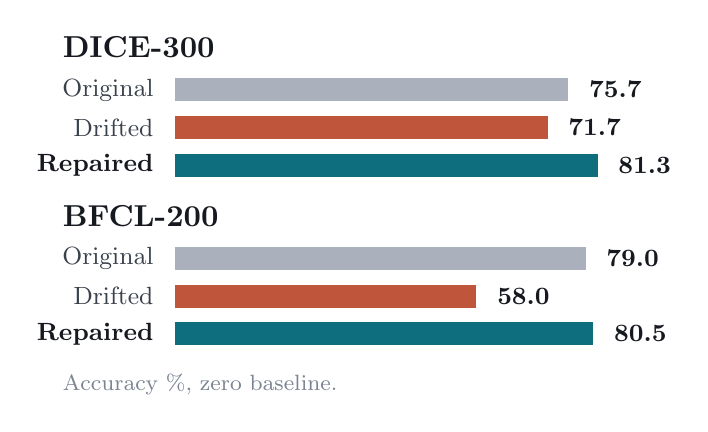
\begin{tikzpicture}[x=1cm,y=1cm]
        \node[anchor=west,text=Ink,font=\bfseries\fontsize{10.5}{13}\selectfont] at (-1.55,3.86) {DICE-300};
        \barrow{3.32}{Original}{75.7}{4.996}{Slate}
        \barrow{2.84}{Drifted}{71.7}{4.732}{Warm}
        \barrowhi{2.36}{Repaired}{81.3}{5.366}{Accent}

        \node[anchor=west,text=Ink,font=\bfseries\fontsize{10.5}{13}\selectfont] at (-1.55,1.72) {BFCL-200};
        \barrow{1.18}{Original}{79.0}{5.214}{Slate}
        \barrow{0.70}{Drifted}{58.0}{3.828}{Warm}
        \barrowhi{0.22}{Repaired}{80.5}{5.313}{Accent}

        \node[anchor=north west,text=Mute,font=\fontsize{8.5}{11}\selectfont] at (-1.55,-0.16)
          {Accuracy \%, zero baseline.};
      \end{tikzpicture}
    \end{column}

    \begin{column}{0.30\textwidth}
      \vspace{0.02cm}
      \stat{19/22}{DICE drift failures recovered}
      \vspace{0.24cm}
      \stat{33/45}{BFCL drift failures recovered}
      \vspace{0.24cm}
      \stat{0}{observed repair harms on originally-correct calls}
    \end{column}
  \end{columns}

  \note{%
    7:00-9:00. Lead with the result. DICE 75.7 to 71.7 to 81.3. BFCL 79.0 to 58.0 to 80.5, so drift damage is far larger there. The counts on the right cover only examples that were correct before drift and then failed. Say "zero observed harms in these slices", not "repair can never harm". Explain that repaired can exceed original because repair also patches some pre-existing baseline misses.\\
    [Sources] Paper 15, Table 1 and Section 6.1.
  }
\end{frame}

% == 8 == Baselines =============================================================
\begin{frame}{A second attempt does not explain it}
  \renewcommand{\barfont}{\fontsize{8.5}{11}\selectfont}%
  \vspace{0.34cm}
  \begin{columns}[T,onlytextwidth]
    \begin{column}{0.475\textwidth}
      {\color{Ink}\fontsize{12}{15}\selectfont\bfseries DICE-300\par}
      \vspace{0.30cm}
      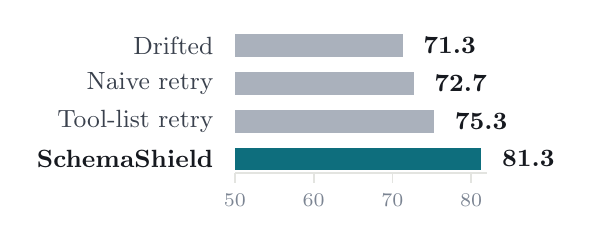
\begin{tikzpicture}[x=1cm,y=1cm]
        \foreach \xx/\lab in {0/50,1.00/60,2.00/70,3.00/80}{%
          \draw[Line,line width=0.6pt] (\xx,-0.06) -- (\xx,-0.19);
          \node[anchor=north,text=Mute,font=\fontsize{7}{9}\selectfont] at (\xx,-0.20) {\lab};}
        \draw[Line,line width=0.6pt] (0,-0.06) -- (3.20,-0.06);
        \barrow{1.56}{Drifted}{71.3}{2.130}{Slate}
        \barrow{1.08}{Naive retry}{72.7}{2.270}{Slate}
        \barrow{0.60}{Tool-list retry}{75.3}{2.530}{Slate}
        \barrowhi{0.12}{SchemaShield}{81.3}{3.130}{Accent}
      \end{tikzpicture}
    \end{column}
    \begin{column}{0.475\textwidth}
      {\color{Ink}\fontsize{12}{15}\selectfont\bfseries BFCL-200\par}
      \vspace{0.30cm}
      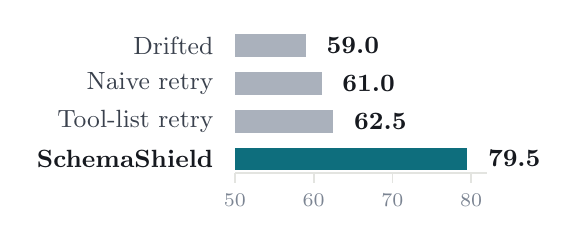
\begin{tikzpicture}[x=1cm,y=1cm]
        \foreach \xx/\lab in {0/50,1.00/60,2.00/70,3.00/80}{%
          \draw[Line,line width=0.6pt] (\xx,-0.06) -- (\xx,-0.19);
          \node[anchor=north,text=Mute,font=\fontsize{7}{9}\selectfont] at (\xx,-0.20) {\lab};}
        \draw[Line,line width=0.6pt] (0,-0.06) -- (3.20,-0.06);
        \barrow{1.56}{Drifted}{59.0}{0.900}{Slate}
        \barrow{1.08}{Naive retry}{61.0}{1.100}{Slate}
        \barrow{0.60}{Tool-list retry}{62.5}{1.250}{Slate}
        \barrowhi{0.12}{SchemaShield}{79.5}{2.950}{Accent}
      \end{tikzpicture}
    \end{column}
  \end{columns}

  \vspace{0.78cm}
  \hairline
  \vspace{0.12cm}
  {\fontsize{11}{14}\selectfont\bfseries
    Structured feedback supplies what repetition cannot.\par}

  \note{%
    9:00-10:20. Naive retry repeats the identical drifted prompt. Tool-list retry says the call is invalid and lists names, but withholds the failed call and the validation errors. Both stay far below the full stack, so the gain is not just paying for a second inference call. Flag that the drifted anchor differs slightly from the previous slide because these are separate runs.\\
    [Sources] Paper 15, Section 6.2 and Table 2.
  }
\end{frame}

% == 9 == Which drift hurts =====================================================
\begin{frame}{One distractor does most of the damage}
  \vspace{0.46cm}
  \begin{columns}[T,onlytextwidth]
    \begin{column}{0.56\textwidth}
      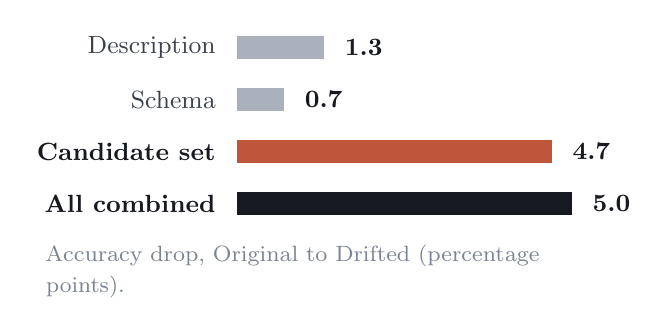
\begin{tikzpicture}[x=1cm,y=1cm]
        \barrow{2.34}{Description}{1.3}{1.105}{Slate}
        \barrow{1.68}{Schema}{0.7}{0.595}{Slate}
        \barrowhi{1.02}{Candidate set}{4.7}{3.995}{Warm}
        \barrowhi{0.36}{All combined}{5.0}{4.250}{Ink}
        \node[anchor=north west,text=Mute,font=\fontsize{8.5}{11}\selectfont,
              text width=7.2cm] at (-2.55,-0.04)
          {Accuracy drop, Original to Drifted (percentage points).};
      \end{tikzpicture}
    \end{column}

    \begin{column}{0.40\textwidth}
      \vspace{0.02cm}
      {\color{Ink}\fontsize{13.5}{16.5}\selectfont\bfseries
        Catalog growth is the failure mode.\par}
      \vspace{0.22cm}
      {\fontsize{10}{13}\selectfont
        One overlapping tool nearly matches the full combined drop. Rewording and renaming barely register.\par}
      \vspace{0.22cm}
      {\color{Mute}\fontsize{9.5}{12.5}\selectfont
        DICE-300, Qwen3.5-9B. Do not generalize this ordering beyond the slice.\par}
    \end{column}
  \end{columns}

  \note{%
    10:20-11:35. Description drift costs 1.3 points, schema drift 0.7. One overlapping distractor costs 4.7, almost the entire 5.0-point combined drop. Keep repeating "in this model and this slice". The transferable point is that catalog growth deserves testing separately from description or schema revisions.\\
    [Sources] Paper 15, Section 6.4 and Table 4.
  }
\end{frame}

% == 10 == Coverage and cost ====================================================
\begin{frame}{Mostly visible, but not free}
  \vspace{0.18cm}
  \begin{columns}[T,onlytextwidth]
    \begin{column}{0.42\textwidth}
      \eyebrow{Validator-visible drift misses}
      \vspace{0.26cm}
      \begin{columns}[T,onlytextwidth]
        \begin{column}{0.46\textwidth}\stat{20/22}{DICE}\end{column}
        \begin{column}{0.46\textwidth}\stat{45/45}{BFCL}\end{column}
      \end{columns}
      \vspace{0.34cm}
      {\fontsize{10.5}{14}\selectfont
        Only two DICE misses slipped through as \emph{schema-valid but wrong}. That is the blind spot --- a validator cannot catch them.\par}
    \end{column}

    \begin{column}{0.52\textwidth}
      \eyebrow{What the reliability costs}
      \vspace{0.24cm}
      \renewcommand{\arraystretch}{1.30}
      {\fontsize{10}{12.5}\selectfont
      \begin{tabular}{@{}>{\RaggedRight\arraybackslash}p{3.85cm}
                        >{\centering\arraybackslash}p{1.25cm}
                        >{\centering\arraybackslash}p{1.25cm}@{}}
        \toprule
        & \textbf{DICE} & \textbf{BFCL} \\
        \midrule
        Repair-stage invocation & 21.0\% & 36.5\% \\
        Relative token overhead & 32.6\% & 47.1\% \\
        Unresolved tool names   & 15     & 9      \\
        \bottomrule
      \end{tabular}}\par
      \vspace{0.24cm}
      {\color{Mute}\fontsize{9.5}{12.5}\selectfont
        The deployment question is whether the gain is worth this trigger rate.\par}
    \end{column}
  \end{columns}

  \note{%
    11:35-13:00. Good news: the validator sees nearly every drift failure on the originally-correct slice, so the repair layer targets the dominant failure mode. The two DICE exceptions are schema-valid but semantically wrong, which is a real blind spot. Then be honest about cost: it fires on 21 to 36.5 percent of examples and adds 32.6 to 47.1 percent tokens in these runs.\\
    [Sources] Paper 15, Sections 6.1 and 6.3.
  }
\end{frame}

% == 11 == Portability ==========================================================
\begin{frame}{Portability tracks tool-name resolution}
  \vspace{0.24cm}
  \renewcommand{\arraystretch}{1.26}
  {\fontsize{10}{12.5}\selectfont
  \begin{tabular}{@{}>{\RaggedRight\arraybackslash}p{3.05cm}
                    >{\centering\arraybackslash}p{1.45cm}
                    >{\centering\arraybackslash}p{1.45cm}
                    >{\centering\arraybackslash}p{1.20cm}
                    >{\RaggedRight\arraybackslash}p{4.25cm}@{}}
    \toprule
    \textbf{BFCL-200 model} & \textbf{Drifted} & \textbf{Repaired} & \textbf{Gain} & \textbf{Reading} \\
    \midrule
    Qwen3.5-9B      & 58.0\% & \textbf{80.5\%} & +22.5 & Primary non-oracle run \\
    Qwen3.5-35B-A3B & 63.5\% & \textbf{84.5\%} & +21.0 & Same-family replication \\
    \addlinespace[0.30em]
    Llama-4-Scout   & 63.5\% & 66.5\%          & +3.0  & 43 tool names never resolve \\
    GPT-4o-mini     & 84.0\% & 86.0\%          & +2.0  & Small, not significant \\
    \bottomrule
  \end{tabular}}\par

  \vspace{0.30cm}
  \hairline
  \vspace{0.10cm}
  {\fontsize{10.5}{13.5}\selectfont
    If the model cannot name a visible tool, a schema-constrained repair has nothing to attach to.\par}

  \note{%
    13:00-14:20. The 35B Qwen replication is strong. Llama gains only 3 points, and the clue is the last column: 43 unresolved names. GPT-4o-mini starts from much less drift damage and its 2-point gain is not significant. State plainly that the strongest evidence stays inside the Qwen family. This is not a model-independent layer.\\
    [Sources] Paper 15, Table 1 and Section 6.7.
  }
\end{frame}

% == 12 == Limits ===============================================================
\begin{frame}{What we do not claim}
  \vspace{0.18cm}
  \begin{columns}[T,onlytextwidth]
    \begin{column}{0.47\textwidth}
      {\color{Warm}\rule{\textwidth}{2pt}\par}
      \vspace{0.14cm}
      \eyebrow{The evidence is narrow}
      \vspace{0.18cm}
      {\fontsize{10}{13}\selectfont
      \begin{itemize}\setlength\itemsep{0.16cm}
        \item Strongest non-oracle results sit in one model family
        \item Llama-4-Scout omits tool names, so recovery stays limited
        \item The GPT-4o-mini gain is not significant
      \end{itemize}}
    \end{column}
    \begin{column}{0.47\textwidth}
      {\color{Slate}\rule{\textwidth}{2pt}\par}
      \vspace{0.14cm}
      \eyebrow{The setting is controlled}
      \vspace{0.18cm}
      {\fontsize{10}{13}\selectfont
      \begin{itemize}\setlength\itemsep{0.16cm}
        \item Drift operators are author-designed, not mined
        \item Ablations are oracle-constrained upper bounds
        \item We score one call, not a sequential tool plan
      \end{itemize}}
    \end{column}
  \end{columns}

  \vspace{0.26cm}
  \hairline
  \vspace{0.10cm}
  {\fontsize{10.5}{13.5}\selectfont
    Strict matching cuts the other way: it makes the reported recovery rates \textbf{conservative}.\par}

  \note{%
    14:20-15:15. Be explicit before the takeaway. The non-oracle evidence concentrates in one family. The drift operators are deployment-motivated and were checked against 11 Notion and Stripe changelog items, but they were not derived from them, and that audit does not estimate how often real changes look like ours. Strict matching makes the recovery rates conservative.\\
    [Sources] Paper 15, Sections 8 and 9; Section 5.3 changelog audit.
  }
\end{frame}

% == 13 == Takeaway =============================================================
\begin{frame}[plain]
  \darkbleed

  \vspace{0.22cm}
  {\color{Accent}\rule{0.55cm}{2pt}}\par
  \vspace{0.20cm}
  \eyebrowon{DarkMute}{Takeaway}

  \vspace{0.78cm}
  {\color{Canvas}\fontsize{24}{28}\selectfont\bfseries
    Treat tool interfaces as\\evolving contracts.\par}

  \vspace{0.46cm}
  {\color{DarkMute}\fontsize{11.5}{15.5}\selectfont
    Validate against the live catalog, retry selection on a missing name,\\
    then constrain one repair.\par}

  \vspace{1.30cm}
  \begin{columns}[b,onlytextwidth]
    \begin{column}{0.68\textwidth}
      {\color{DarkMute}\fontsize{9}{11.5}\selectfont
        Code, prompts, fixed slices, and example-level traces\par}
      \vspace{0.08cm}
      {\color{Canvas}\ttfamily\fontsize{9.5}{12}\selectfont github.com/AniruddhaChattopadhyay/tool-drift\par}
    \end{column}
    \begin{column}{0.30\textwidth}
      \raggedleft{\color{Canvas}\fontsize{19}{22}\selectfont\bfseries Questions?}
    \end{column}
  \end{columns}
  \vspace{0.52cm}

  \note{%
    15:15-16:00. Close by resolving the opening problem. The recipe is live validation, candidate-set retry for a missing name, and constrained repair once a tool is resolved. It works when the failure is visible and the name resolves; it does not help valid-but-wrong calls. Invite questions and leave roughly four minutes.\\
    [Sources] Paper 15, Discussion and Conclusion; artifact repository at commit fbac156.
  }
\end{frame}

% =========================== BACKUP ==========================================
\appendix

% == 14 ==
\begin{frame}{Backup: statistical detail}
  \vspace{0.44cm}
  \renewcommand{\arraystretch}{1.42}
  \setlength{\tabcolsep}{4pt}
  {\fontsize{10}{12.5}\selectfont
  \begin{tabular}{@{}>{\RaggedRight\arraybackslash}p{2.15cm}
                    >{\centering\arraybackslash}p{2.60cm}
                    >{\centering\arraybackslash}p{2.60cm}
                    >{\centering\arraybackslash}p{2.60cm}
                    >{\centering\arraybackslash}p{2.15cm}@{}}
    \toprule
    \textbf{Benchmark} & \textbf{Original} & \textbf{Drifted} & \textbf{Repaired} & \textbf{McNemar $p$} \\
    \midrule
    DICE-300 & 0.757 [.70,.80] & 0.717 [.67,.77] & \textbf{0.813 [.77,.86]} & $3.7\times10^{-9}$ \\
    BFCL-200 & 0.790 [.74,.84] & 0.580 [.51,.65] & \textbf{0.805 [.75,.86]} & $5.7\times10^{-14}$ \\
    \bottomrule
  \end{tabular}}\par

  \vspace{0.54cm}
  {\fontsize{11}{14.5}\selectfont
    Bootstrap intervals support the large repaired-vs-drifted effect. They do \textbf{not} justify strong claims about small gaps between nearby oracle and non-oracle runs.\par}

  \note{[Sources] Paper 15, Table 1 and Section 6.1. 95 percent bootstrap CIs, seed 42.}
\end{frame}

% == 15 ==
\begin{frame}{Backup: validation drives the recovery}
  \vspace{0.22cm}
  \renewcommand{\arraystretch}{1.24}
  {\fontsize{10}{12.5}\selectfont
  \begin{tabular}{@{}>{\RaggedRight\arraybackslash}p{2.15cm}
                    >{\RaggedRight\arraybackslash}p{5.05cm}
                    >{\centering\arraybackslash}p{1.95cm}
                    >{\centering\arraybackslash}p{1.95cm}@{}}
    \toprule
    \textbf{Benchmark} & \textbf{Oracle-constrained variant} & \textbf{Drifted} & \textbf{Repaired} \\
    \midrule
    DICE-300 & Canonical card only         & 0.770 & 0.770 \\
             & Validation + retry, no card & 0.730 & \textbf{0.830} \\
             & Full \method                & 0.713 & 0.827 \\
    \addlinespace[0.30em]
    BFCL-200 & Canonical card only         & 0.810 & 0.810 \\
             & Validation + retry, no card & 0.645 & \textbf{0.820} \\
             & Full \method                & 0.640 & 0.795 \\
    \bottomrule
  \end{tabular}}\par

  \vspace{0.30cm}
  {\fontsize{10.5}{13.5}\selectfont
    The card alone recovers nothing. Validation plus retry does the work --- the card earns its keep earlier, as \emph{drift prevention} at the initial prediction step.\par}

  \note{[Sources] Paper 15, Section 6.5 and Table 5. Oracle-constrained mechanism evidence, not deployment-facing.}
\end{frame}

% == 16 ==
\begin{frame}{Backup: residual failure modes}
  \vspace{0.20cm}
  \begin{columns}[T,onlytextwidth]
    \begin{column}{0.47\textwidth}
      \eyebrow{Non-oracle residuals}
      \vspace{0.24cm}
      {\fontsize{10.5}{14}\selectfont
      \begin{itemize}\setlength\itemsep{0.20cm}
        \item Missing fields still missing after repair
        \item Tool names that never resolve
        \item Two DICE calls that are schema-valid but wrong
      \end{itemize}}
    \end{column}
    \begin{column}{0.47\textwidth}
      \eyebrow{Strict-match artifacts}
      \vspace{0.16cm}
      \stat{11/13}{inspected misses were formatting or paraphrase mismatches}
      \vspace{0.26cm}
      {\fontsize{10.5}{14}\selectfont
        So exact-match recovery is \textbf{conservative} for those inspected cases.\par}
    \end{column}
  \end{columns}

  \note{[Sources] Paper 15, Section 6.6 and Table 6. Small inspected set: evidence of an evaluation artifact, not a replacement accuracy estimate.}
\end{frame}

% == 17 ==
\begin{frame}{Backup: reproducibility}
  \vspace{0.36cm}
  \begin{columns}[T,onlytextwidth]
    \begin{column}{0.54\textwidth}
      {\fontsize{10.5}{14}\selectfont
      \begin{itemize}\setlength\itemsep{0.18cm}
        \item Fixed benchmark slices and drift configurations
        \item Prompts, scoring logic, normalized semantic matching
        \item Per-example outputs and validation traces
        \item Repair targets, strategies, token usage, raw artifacts
      \end{itemize}}
    \end{column}
    \begin{column}{0.42\textwidth}
      \vspace{0.06cm}
      \eyebrow{Artifact}
      \vspace{0.20cm}
      {\color{Ink}\ttfamily\fontsize{10}{13.5}\selectfont
        github.com/\\AniruddhaChattopadhyay/\\tool-drift\par}
      \vspace{0.24cm}
      {\color{Mute}\fontsize{9.5}{12.5}\selectfont Commit \texttt{fbac156}\par}
    \end{column}
  \end{columns}

  \note{[Sources] Paper 15, Section 5.6 and the artifact repository.}
\end{frame}

\end{document}
